\myChapter{Nuztungsm\"oglichkeiten}\label{chap:concept}
In diesem Kapitel soll ein kurzer Überblick über verschiedene
Anwendungsmöglichkeiten der in dieser Arbeit vorgestellten Service Engine und der
Service Implementierungen gegeben werden. Grundsätzlich sind auch andere
Anwendungsszenarios denkbar, denn vor allem in der Integration mit anderen
Anwendungen hat die Service Engine als protokollunabhängige Ausführungsschicht
erhebliche Vorteile. So können bei Bedarf jederzeit neue Protocol Handler
angebunden werden, ohne dass die Anwendungslogik angepasst werden muss.

\section{Service Klassenbibliothek}
In Kapitel \ref{chap:servicelayer} wurde eine Art des Presentation Layer
vorgestellt, der die Anwendungslogik des Service Layer über verschiedene \ac{RPC}
Protokolle verfügbar macht und deshalb Remoting Layer genannt wurde.
Entsprechend dem Prinzip einer Schichtenarchitektur sind aber auch andere Formen
des Presentation Layer möglich. Dabei können die in Kapitel
\ref{chap:servicelayer} vorgestellten Service Implementierungen
weiterhin verwendet werden. Eine Möglichkeit wäre beispielsweise ein
Presentation Layer in Form einer Weboberfläche. Dabei sind die Service
Implementierungen eine Grundlage für den Service Layer der Webapplikation.

Da die Service Implementierungen bereits stark von den Möglichkeiten des Spring
Framework gebrauch machen, bietet sich das \ac{MVC} Modul des Spring Frameworks
an, das die Erstellung von Webapplikationen auf Basis des Spring Frameworks
erlaubt. Auch die Verwendung des Groovy Webframeworks Grails wäre denkbar, da es
ebenfalls auf dem Spring \ac{MVC} Framework aufbaut und einige der Services in
Groovy implementiert wurden. So lange die Groovy Laufzeitbibliotheken für die
Service Implementierungen verfügbar sind, ist eine direkte Verwendung von Groovy
aber nicht notwendig. Die nachfolgende Abbildung \ref{ill:springmvc} zeigt eine
Möglichkeit für die Architektur einer Webapplikatione, die die Service
Implementierungen und das Spring \ac{MVC} Modul verwendet.

\begin{figure}
    \center{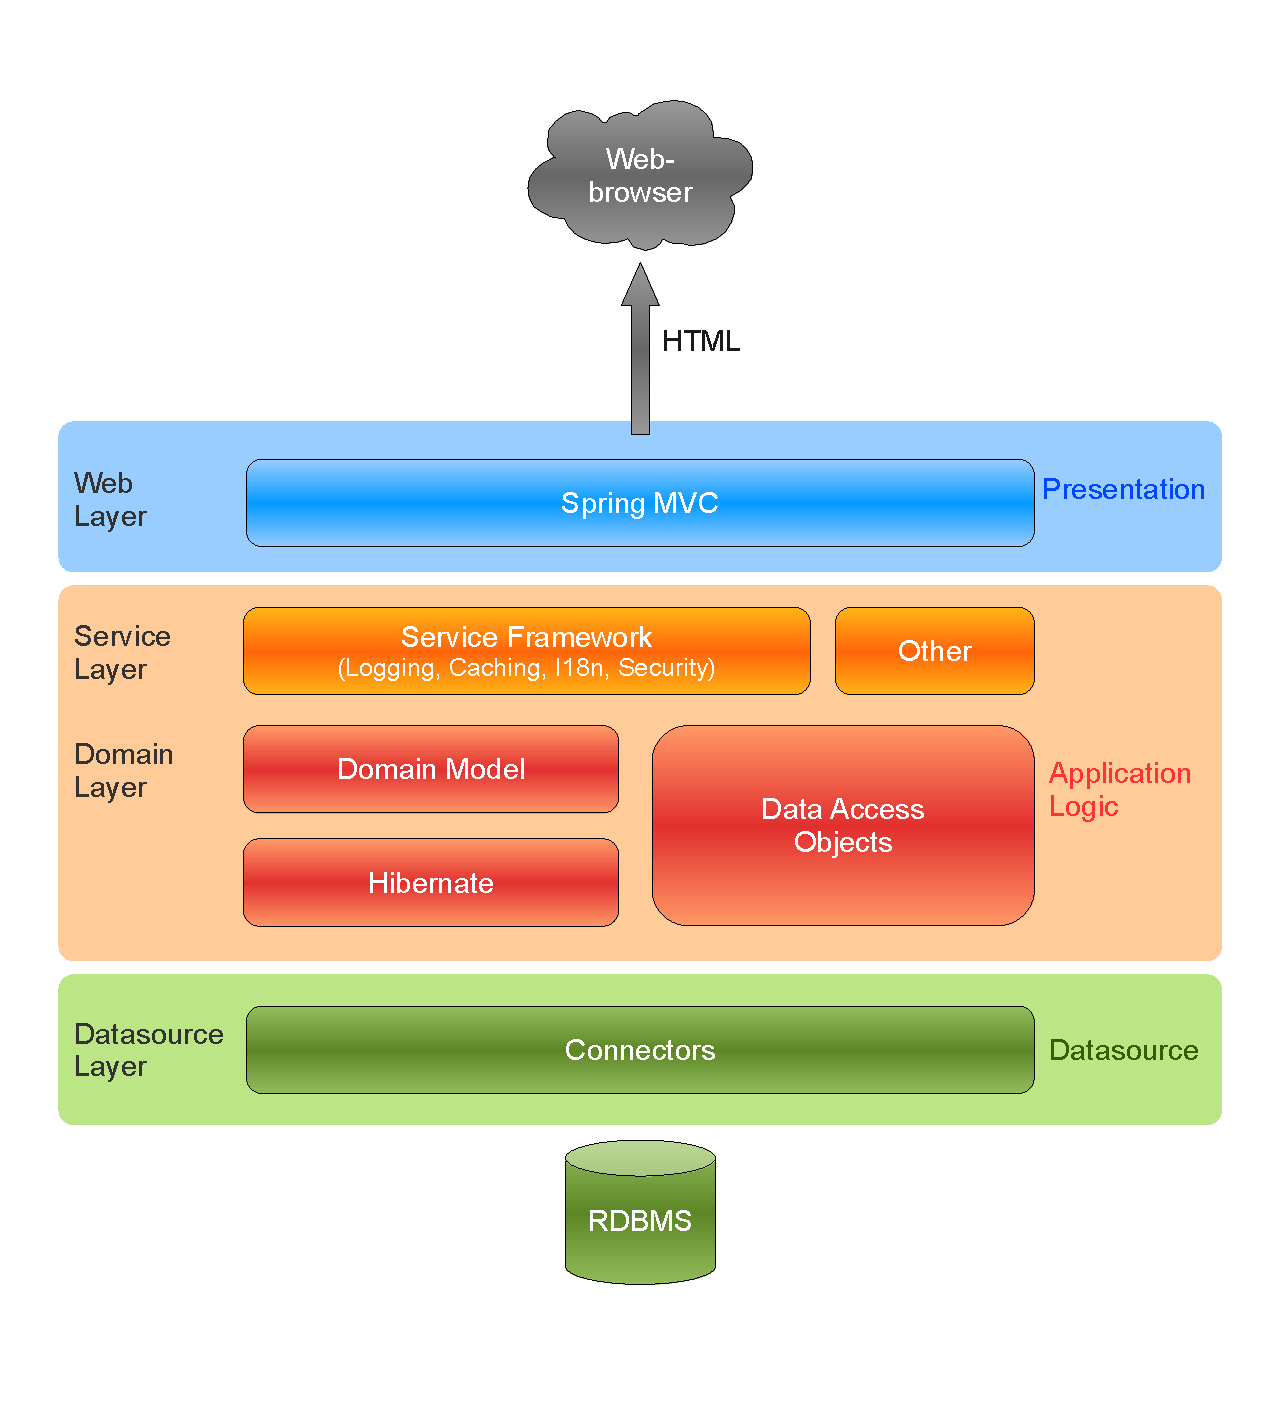
\includegraphics[width=\linewidth]{images/overviews/uc_springmvc}}
    \caption{Verwendung der Service Implementierungen in einer Spring MVC
    Webanwendung}
	\label{ill:springmvc}
\end{figure}

\pagebreak
\section{Rich Internet Applications}
Eine \ac{RIA} ist eine Webanwendung, die ähnlich wie eine klassische
Desktopapplikation zu bedienen ist (siehe \cite{wiki:ria}). Typischerweise wird
für die Verwendung dieser Anwendungen ein Browser Plugin\footnote{Beispielsweise
für Java, Microsoft Silverlight oder Adobe Flash} benötigt, aber auch klassische
Webapplikationen, die die Benutzeroberfläche zum Großteil durch JavaScript
dynamisch gestalten fallen inzwischen in diese Kategorie. Eine \ac{RIA}
übernimmt die Aufgabe der Darstellung von Daten und kommuniziert dann mit einem
Webserver, der für die Datenhaltung zuständig ist.
 
Da viele \ac{RIA} Frontends in ECMAScript Derivaten wie JavaScript oder
ActionScript\footnote{Verwendet in Adobe Flash, Adobe Flex und Adobeb Air}
entwickelt werden, ist die Kombination aus \ac{REST} mit \ac{HTTP} als
Übertragungsprotokoll und \ac{JSON} als Austauschformat für die Kommunikation mit
dem Server sehr beliebt. Aus diesem Grund bietet es sich an, die Service Engine
in Verbindung mit dem \ac{REST} Protocol Handler und den in Kapitel
\ref{chap:servicelayer} vorgestellten Service Funktionalitäten zu verwenden.
Durch diesen Aufbau lässt sich schnell eine serverseitige Grundlage für die
Verwendung in \ac{RIA} Anwendungen schaffen.

Ein weiterer Vorteil der Service Engine ist dabei, dass andere Anwendungen
weiterhin über ihr bevorzugtes Protokoll kommunizieren können. So ist für eine
Java Anwendung die Kommunikation über \ac{RMI} deutlich einfacher und
performanter und sollte deshalb wenn möglich auch verwendet werden. Abbildung
\ref{ill:rias} zeigt eine Übersicht, wie eine \ac{RIA} mit der Service Engine
kommuniziert und wie eine Java Anwendung passend angebunden werden kann.

\begin{figure}
    \center{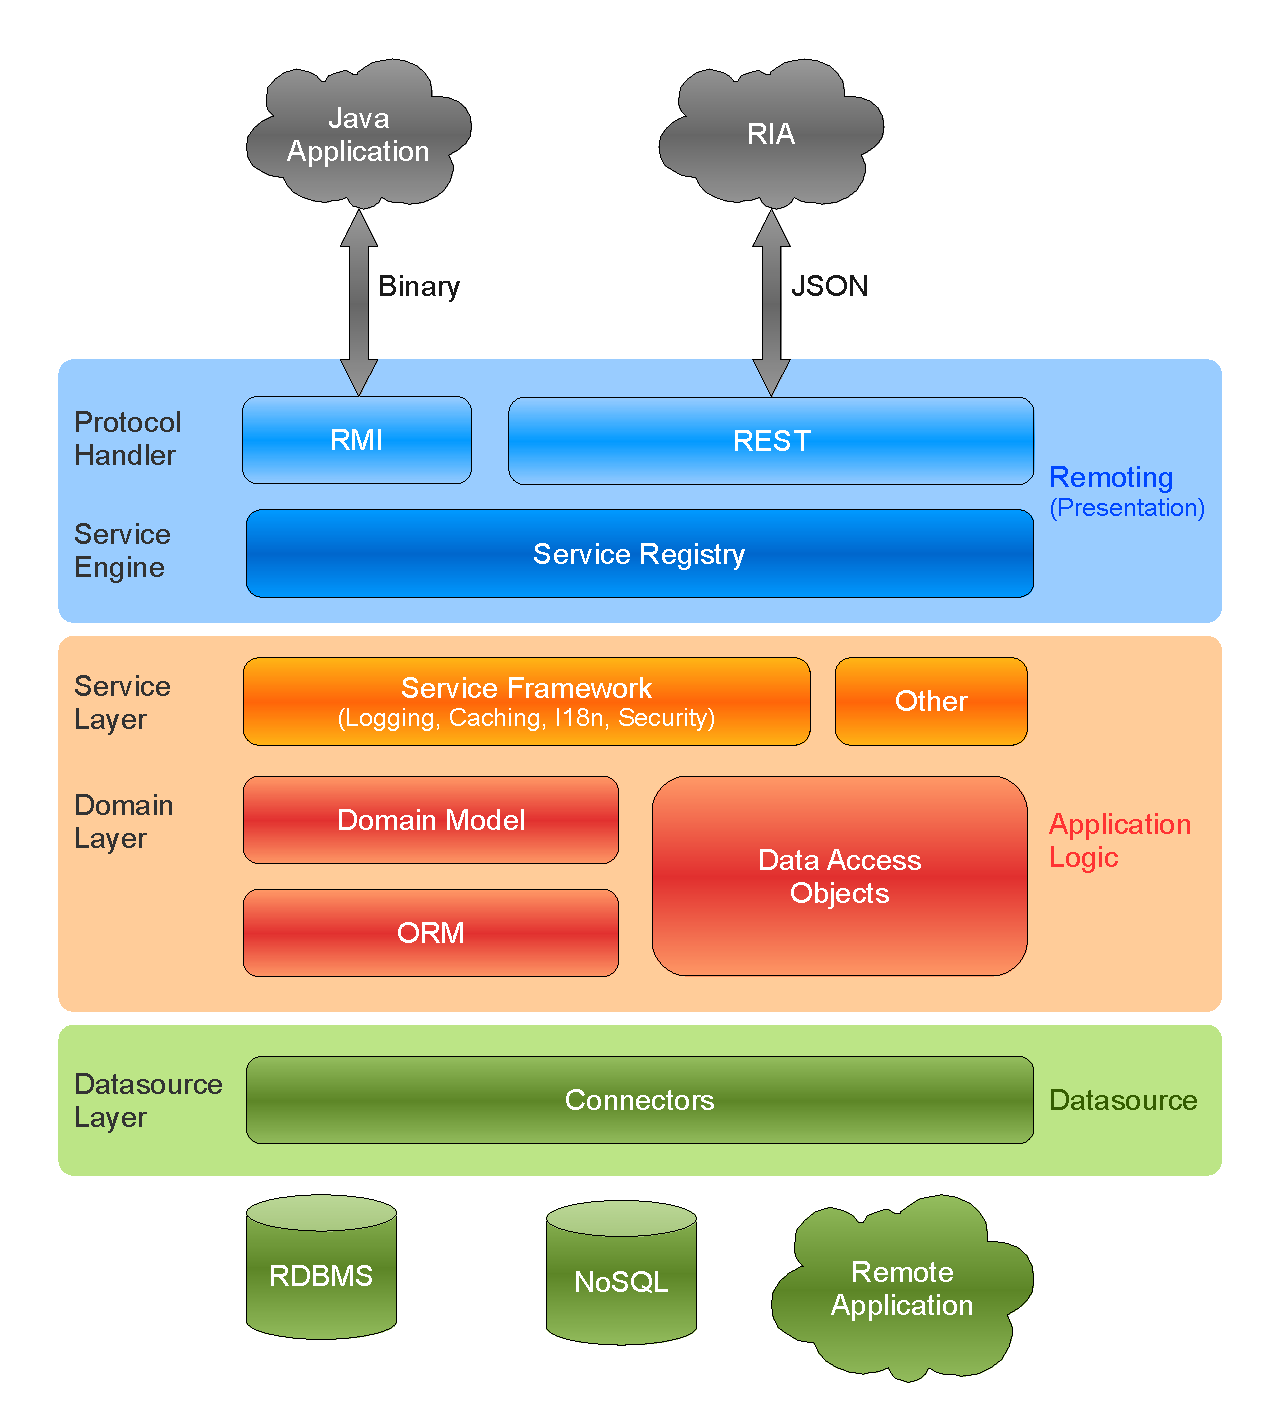
\includegraphics[width=\linewidth]{images/overviews/uc_ria}}
	\caption{Übersicht für die Verwendung mit Rich Internet Applications}
	\label{ill:rias}
\end{figure}

\pagebreak
\section{Gateway}
Grundsätzlich stellt eine Anwendung die Verbindung mit anderen entfernten
Systemen im Datasource Layer her. Die \ac{DAO} Implementierungen übernehmen dann
die Aufgabe über diese Verbindung Anfragen an ein entferntes System zu stellen
und die Ergebnisse in das Domain Model der Anwendung zu konvertieren, wo es weiter
verarbeitet wird. In manchen Fällen kann es aber auch sinnvoll sein, die
Methoden des Entfernten Systems direkt als Service Interface zur Verfügung zu stellen. Die
Implementierung dieses Interface leitet dann alle Methodenaufrufe direkt an das
entfernte System weiter und übernimmt somit die Aufgabe einer Gateway. Eine
Gateway arbeitet hierbei als Vermittler zwischen dem aufrufenden Client und einem
anderen entfernten System, wobei der Client lediglich Kenntnis über das System
benötigt mit dem er direkt kommuniziert, in diesem Fall also der Service Engine
und dem Service Interface. Der Vorteil hierbei ist, dass ein Client ein
beliebiges von den verwendeten Protocol Handlern angebotenes \ac{RPC}
Protokoll verwenden kann. Somit kann ein entferntes System über
Protokolle angebunden werden, die von diesem nicht direkt unterstützt werden.

Die Implementierung einer verallgemeinerten Gateway Funktionalität befindet sich
noch in einem sehr frühen Stadium, weshalb ein Entwickler momentan einen
Großteil der Konvertierungsarbeit selbst in der entsprechenden Service Implementierung
übernehmen muss. Abbildung \ref{ill:gateway} ordnet die Gateway
Funktionalität in die Gesamtarchitektur einer Anwendung ein.

\begin{figure}
    \center{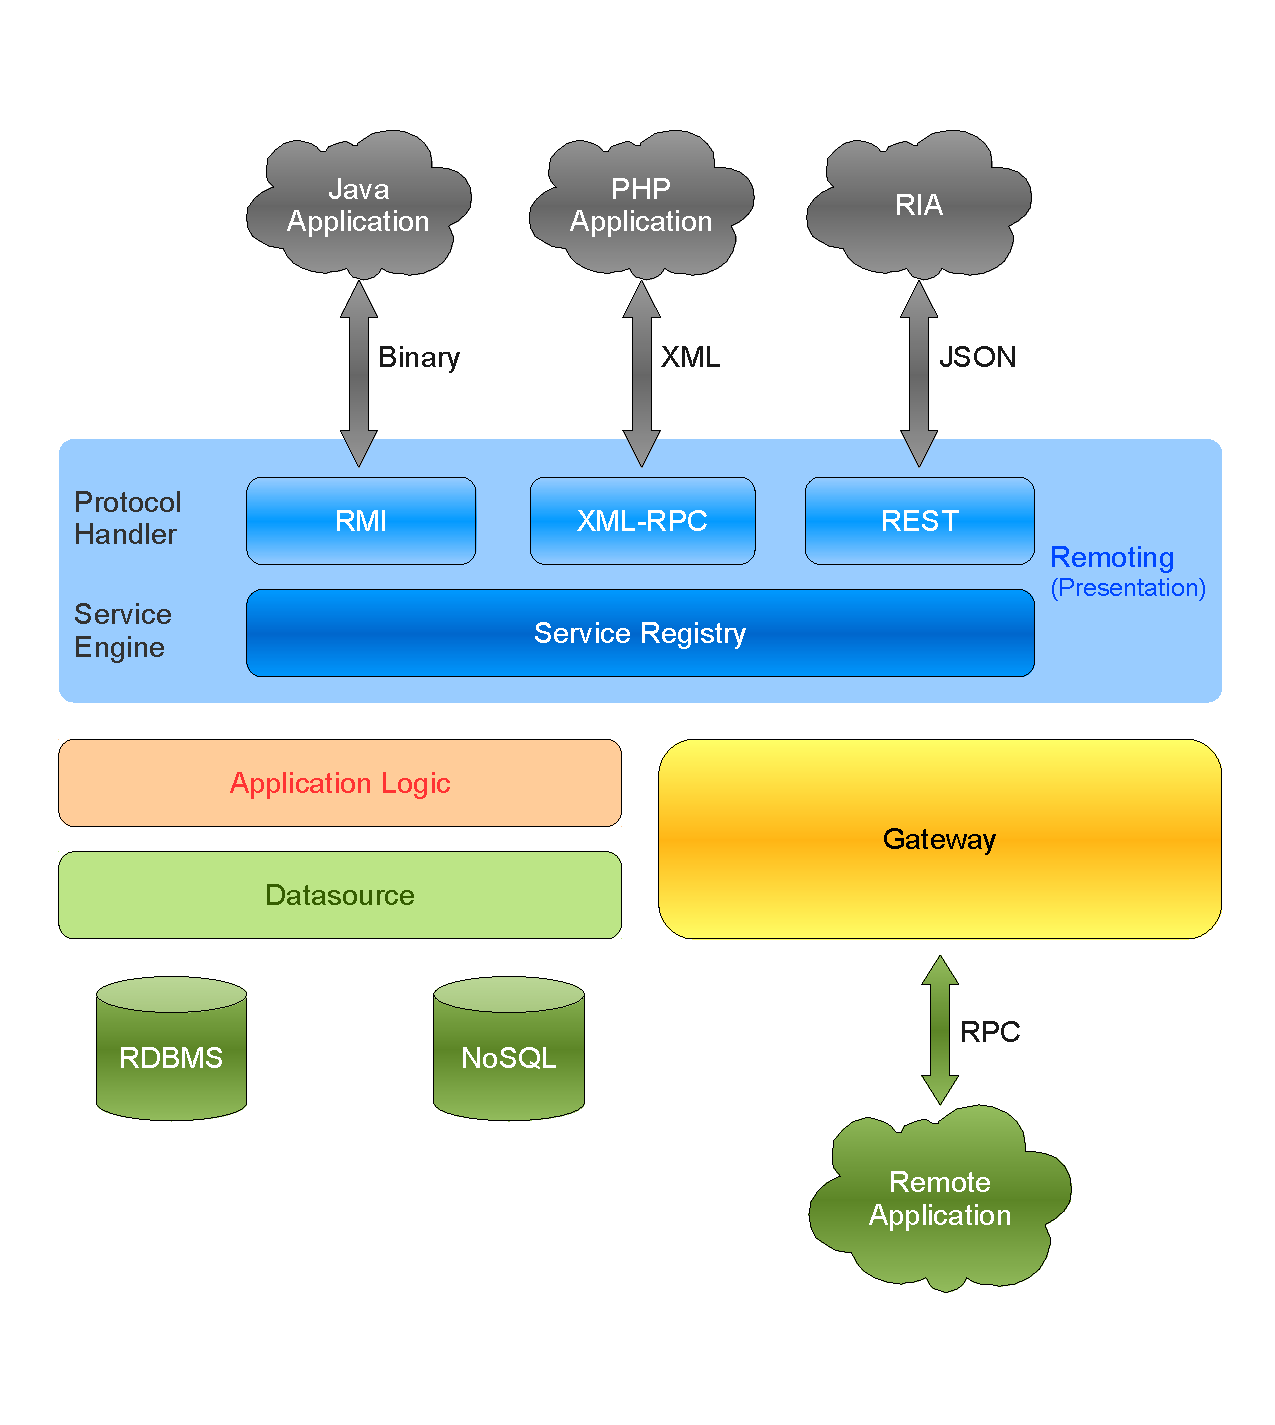
\includegraphics[width=\linewidth]{images/overviews/uc_gateway}}
	\caption{Einordnung der Gateway Funktionalität}
	\label{ill:gateway}
\end{figure}